\section{Výber algoritmu}
\label{kap:3}
Hlavnou časťou našej práce je implementácia algoritmu na hľadanie trajektórie pre pohyb objektu v priestore. Výber správneho algoritmu je preto kľúčový. Je nevyhnutné vybrať taký algoritmus, ktorý najlepšie zodpovedá našej úlohe.

Pri rozhodovaní o vhodnom algoritme je dôležité zohľadniť nielen schopnosť algoritmu nájsť optimálnu trajektóriu, ale aj jeho rýchlosť výpočtu. Vzhľadom na to, že náš robotický systém pracuje v reálnom čase, je kľúčové zvoliť algoritmus, ktorý dokáže rýchlo generovať trajektórie bez zbytočného oneskorenia.

V tejto kapitole sa budeme bližšie venovať algoritmu plánovania trajektórie, ktorý sme sa rozhodli zvoliť na riešenie nášho problému a vysvetlíme si dôvody jeho výberu. Taktiež si predstavíme existujúce riešenie, na ktorom budeme v našej práci stavať, rozširovať a upravovať ho podľa potrieb našej úlohy. Na záver si vysvetlíme, ako budeme pristupovať k plánovaniu trajektórie pri jednotlivých kinematických štruktúrach, ktoré budeme testovať.

\subsection{RRT}

Analýzou jednotlivých typov algoritmov pre plánovanie trajektórie sme dospeli k záveru, že najvhodnejšou voľbou pre našu úlohu bude RRT algoritmus. Tento výber sme urobili najmä pre jeho schopnosť rýchlo prehľadávať konfiguračný priestor. RRT algoritmus je vhodný nielen pre svoju rýchlosť, ale aj pre jeho univerzálnosť, pretože ho vieme využiť ako v kartézskom súradnicovom systéme, tak aj v kĺbovej súradnicovej sústave. Táto flexibilita bude dôležitá pri implementácii plánovania trajektórie pre rôzne kinematické štruktúry.

Ďalšou výhodou RRT algoritmu je jeho jednoduchá a rýchla modifikovateľnosť podľa našich potrieb. V našej práci budeme tiež porovnávať RRT algoritmus s jeho modifikáciou, RRT*. Budeme sa snažiť nájsť optimálne riešenie z hľadiska času výpočtu a kvality výslednej trajektórie.


\subsection{Riešenie RRT - python}
RRT algoritmus je široko využívaný a populárny, a preto existuje mnoho dostupných implementácií v rôznych programovacích jazykoch. V našej práci budeme pracovať v jazyku Python, preto sme sa rozhodli analyzovať rôzne voľne dostupné implementácie tohto algoritmu v tomto jazyku.

Z dostupných riešení a implementácií RRT algoritmu v jazyku Python sme sa rozhodli použiť implementáciu od autorov knižnice rrt-algorithms \cite{RRT-python}. Obsahuje samotný RRT algoritmus (obr. \ref{OBRAZOK 3.1}) ako aj jeho modifikácie - RRT* (obr. \ref{OBRAZOK 3.2}) a RRT connect (obr. \ref{OBRAZOK 3.3}).

\begin{figure}[]
	\centering
	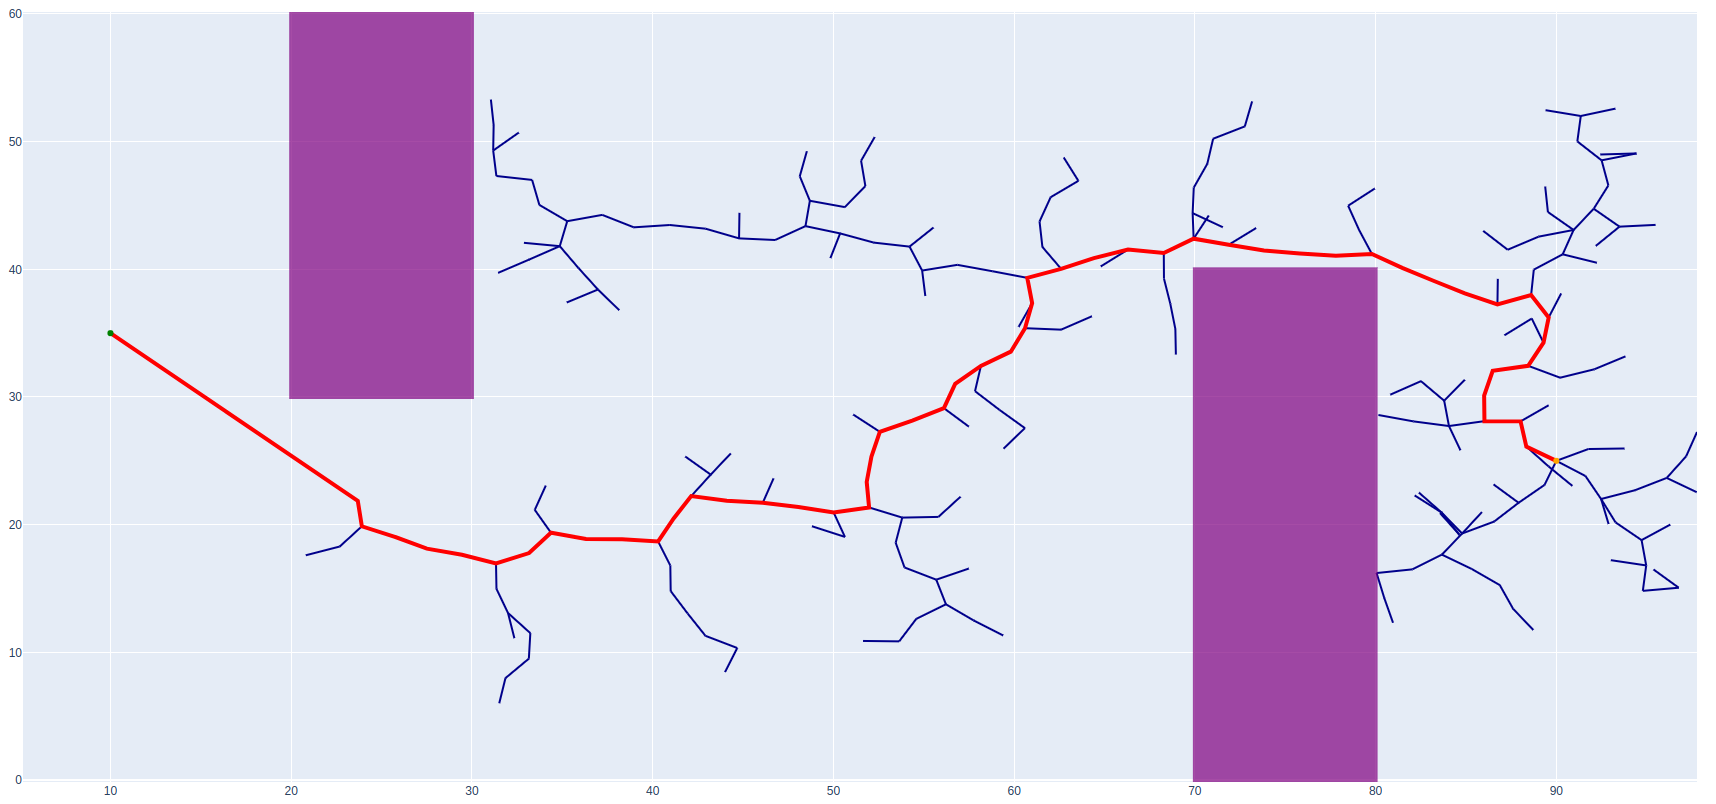
\includegraphics[width=140mm]{img/RRT-2D.png}
	\caption{RRT - dvojrozmerný priestor} \label{OBRAZOK 3.1} 
\end{figure} 
Riešenie, na ktorom budeme stavať, je vytvorené pre plánovanie v kartézskom súradnicovom systéme a to v dvoj aj v trojrozmernom priestore (obr. \ref{OBRAZOK 3.4}). Algoritmu je potrebné zadať rozsah prehľadávaného priestoru, počiatočný a koncový bod a ak sa v priestore nachádzajú prekážky, ich pozície v prehľadávacom priestore. Ako možeme vidieť na obrázkoch \ref{OBRAZOK 3.1}, \ref{OBRAZOK 3.2}, \ref{OBRAZOK 3.3}, táto implementácia pracuje iba s hmotným bodom, neuvažuje teda rozmery prenášaného objektu.
\begin{figure}[]
	\centering
	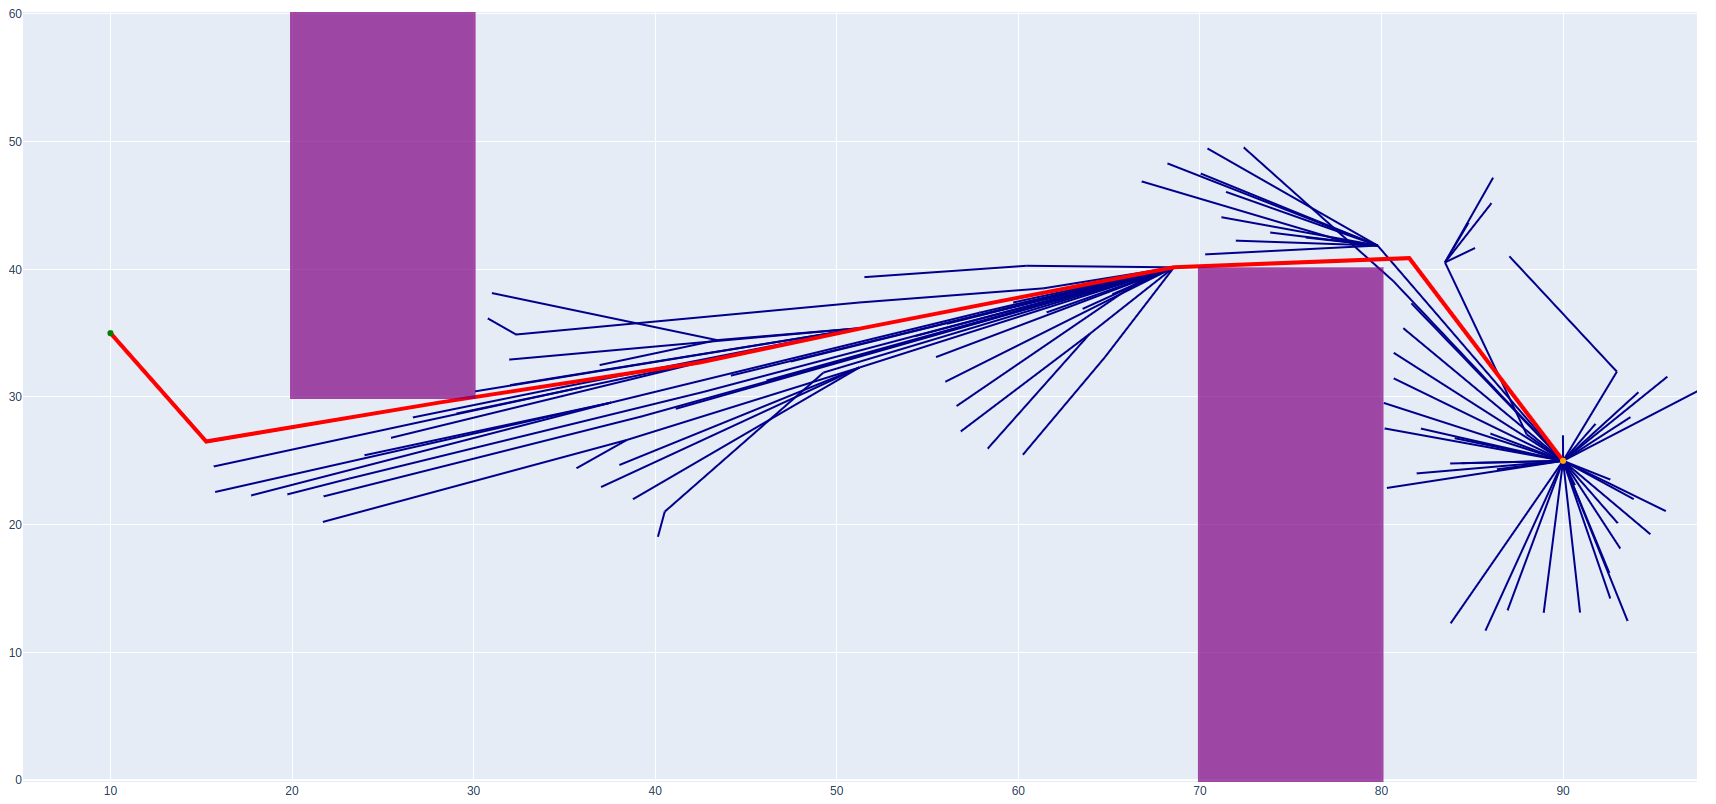
\includegraphics[width=140mm]{img/RRTstar-2D.png}
	\caption{RRT* - dvojrozmerný priestor} \label{OBRAZOK 3.2} 
\end{figure} 

\begin{figure}[]
	\centering
	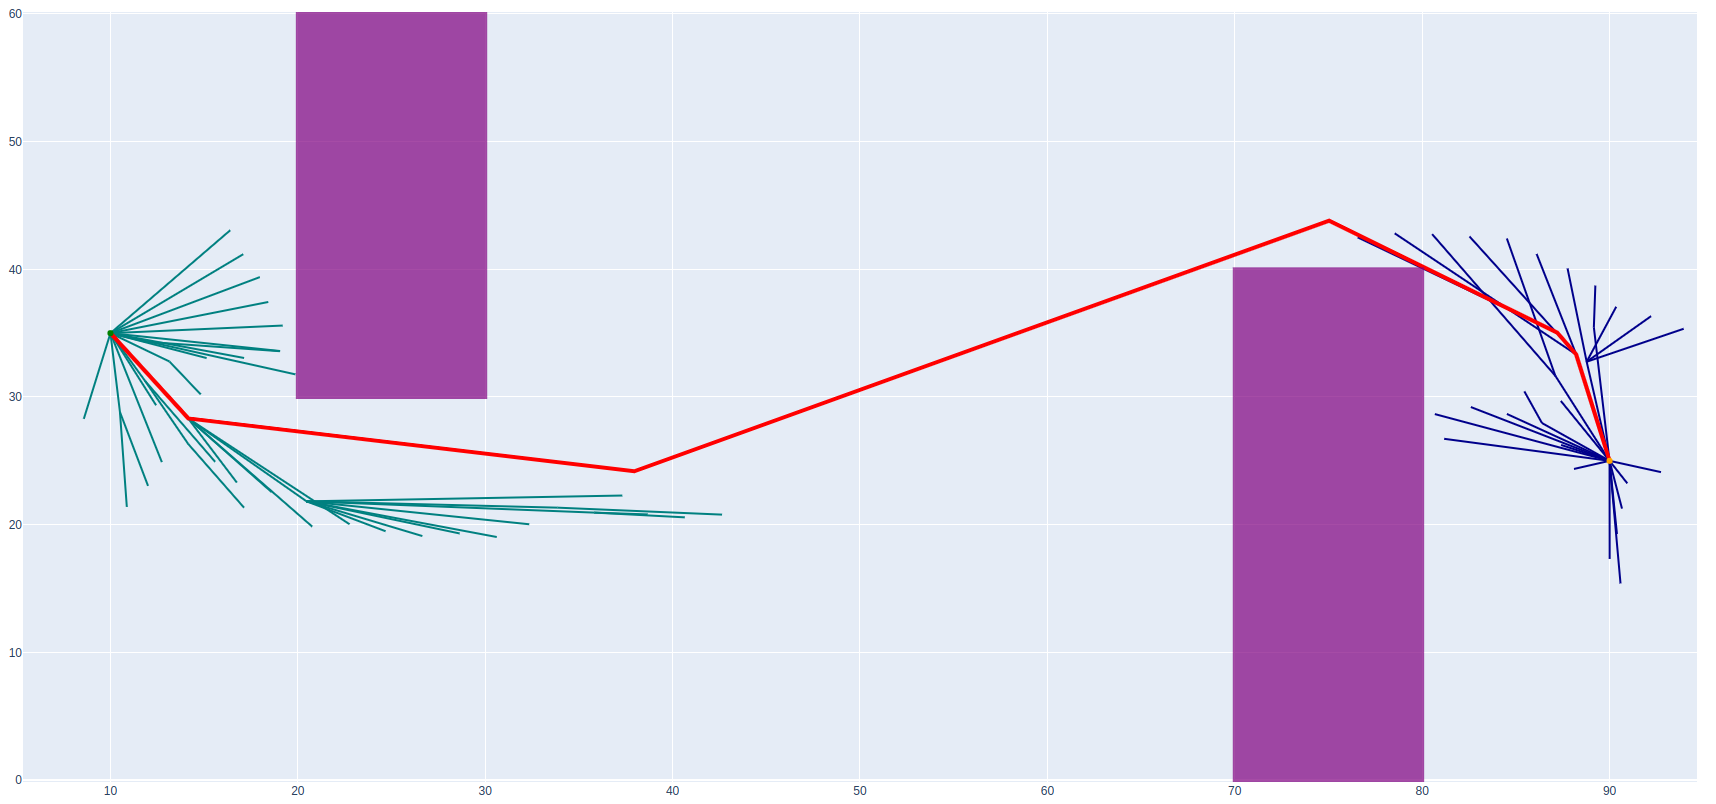
\includegraphics[width=140mm]{img/RRTconnect-2D.png}
	\caption{RRT connect - dvojrozmerný priestor} \label{OBRAZOK 3.3} 
\end{figure} 

\begin{figure}[]
	\centering
	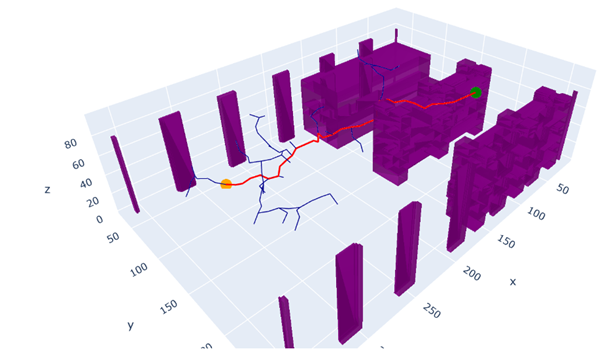
\includegraphics[width=140mm]{img/RRT-3D.png}
	\caption{RRT - trojrozmerný priestor} \label{OBRAZOK 3.4} 
\end{figure} 

Pre riešenie našej úlohy bude potrebné rozšíriť tento algoritmus tak, aby neuvažoval o prenášanom objekte ako o hmotnom bode, ale aby bral do úvahy aj jeho rozmery. Prístup, ktorý je možné zvoliť je kontrola kolízii v generovaných bodoch na základe ktorej bude tento bod uznaný za nevyhovujúci a bude generovaná nová bezkolízna konfigurácia. Objekt bude v priestore definovaný bodom, v ktorom je uchopený robotickým ramenom - v našom prípade to bude geometrický stred objektu, a jeho orientáciou v priestore.  Stred bude definovaný súradnicami $ x $, $ y $ pracovného priestoru v kartézskom súradnicovom systéme. Orientácia objektu bude reprezentovaná ako uhol medzi osou objektu a osou  $x$ v stupňoch.

Plánovanie bude prebiehať na rozdielnych kinematických štruktúrach, preto je dôležité zvoliť správny prístup pre každú z nich a prispôsobiť algoritmus ich individuálnym potrebám.

 
\subsubsection{3 stupne voľnosti}

Plánovanie trajektórie pri kinematickej štruktúre s 3 stupňami voľnosti budeme riešiť primárne v kartézskom súradnicovom systéme. Pre implementáciu nášho algoritmu použijeme RRT v trojrozmernom konfiguračnom priestore, pričom osi $x$ a $y$ budú reprezentovať osi $x$ a $y$ v pracovnom priestore robota. Os $z$ konfiguračného priestoru bude zodpovedať natočeniu objektu okolo jeho stredu, ktorý nám bude reprezentovať bod uchytenia objektu. Rozsah konfiguračného priestoru (tab. \ref{table 3.1}) bude zodpovedať rozsahu pracovnému priestoru robota v osiach $x$, $y$ a rozsahu maximálnej rotácie objektu v priestore.

\begin{table}[h!]
	\centering
	\begin{tabular}{|c|c|c|}
		\hline
		\multicolumn{1}{|l|}{x {[}mm{]}}  & \multicolumn{1}{l|}{y {[}mm{]}} & \multicolumn{1}{l|}{z {[}\degree{]}} \\ \hline
		0 - 1050                                              & 0 - 745                                             & 0 - 360                              \\ \hline

	\end{tabular}
	\caption{Rozsah konfiguračného priestoru - kartézsky súradnicový systém}\label{table 3.1} 
\end{table}

Pri kinematickej štruktúre s 3 stupňami voľnosti budeme tiež testovať plánovanie trajektórie v kĺbovom priestore. Tieto dáta budeme neskôr používať na porovnanie plánovania trajektórie v kĺbovom a kartézskom priestore. Budeme sledovať čas výpočtu algoritmu, úspešnosť nájdenia cesty a kvalitu trajektórie.

Plánovanie trajektórie v kĺbovom priestore nám umožní preskúmať, ako dobre sa algoritmus dokáže prispôsobiť špecifikám kinematickej štruktúry robota a aký vplyv má voľba priestoru na výslednú trajektóriu. Porovnanie výsledkov s plánovaním trajektórie v kartézskom priestore nám poskytne ucelený obraz o výkonnosti a efektívnosti oboch prístupov.

Osi konfiguračného priestoru $x$,$y$ a $z$ budú odpovedať otočeniam jednotlivých kĺbov robotického ramena (tab. \ref{table 3.2}) .
\begin{table}[h]
	\centering
	\begin{tabular}{|c|c|c|}
		\hline
		\multicolumn{1}{|l|}{x {[}\degree{]}}  & \multicolumn{1}{l|}{y {[}\degree{]}} & \multicolumn{1}{l|}{z {[}\degree{]}} \\ \hline
		0 - 180                                             & 0 - 360                                             & 0 - 360                              \\ \hline
		
	\end{tabular}
	\caption{Rozsah konfiguračného priestoru - kĺbový súradnicový systém}\label{table 3.2} 
\end{table}



\subsubsection{2 stupne voľnosti}


Plánovanie trajektórie pri štruktúre s 2 stupňami voľnosti, ktoré predstavujú 2 rotačné kĺby robotického ramena, nám neumožňuje plánovať v kartézskom priestore, pretože nie každá konfigurácia by bola dosiahnuteľná. Z tohto dôvodu je nevyhnutné použiť plánovanie v kĺbovom konfiguračnom priestore. Pôjde o dvojrozmerný konfiguračný priestor, kde osi $x$ a $y$ budú predstavovať rotácie jednotlivých kĺbov. Rozsah konfiguračného priestoru, ktorý odpovedá rozsahu pohybu jednotlivých kĺbov je uvedený v tabuľke \ref{table 3.2}.

\begin{table}[h]
	\centering
	\begin{tabular}{|c|c|c|}
		\hline
		\multicolumn{1}{|l|}{x {[}\degree{]}}  & \multicolumn{1}{l|}{y {[}\degree{]}} \\ \hline
		0 - 180                                             & 0 - 360       \\ \hline
		
	\end{tabular}
	\caption{Rozsah konfiguračného priestoru - kĺbový priestor}\label{table 3.3} 
\end{table}




